\documentclass[a4paper,10pt]{article}
\usepackage[T1]{fontenc}
\usepackage[utf8]{inputenc}
\usepackage[english]{babel}
\usepackage{ae}
\usepackage[a4paper]{geometry}
\usepackage{amsmath}
\usepackage{url}

% package for inline figures not contained in debian
%\usepackage{floatflt}

\usepackage{fancyhdr}
\usepackage{fancyref}
\usepackage{listings}
\usepackage{booktabs}
\usepackage[perpage]{footmisc}
\usepackage{graphicx} 
\usepackage{hyperref}


% Header and Footer Style
\pagestyle{fancy}
\fancyhead{}
\fancyhead[R]{\slshape Malte Rohde}
\fancyhead[L]{\slshape\nouppercase{\rightmark}}
\fancyfoot{}
\fancyfoot[C]{\thepage}
\renewcommand{\headrulewidth}{0pt}
\renewcommand{\sectionmark}[1]{\markright{\thesection\ #1}} 

% No identation
\setlength\headheight{15pt}
\setlength\parindent{0pt} 

% custom commands
\newcommand\parbig{\par\bigskip}
\newcommand\parmed{\par\medskip}
\newcommand{\mailto}[1]{\href{mailto:#1}{#1}}

% Listing environment for C
\lstnewenvironment{code}[1][]%
  {\minipage{\linewidth} 
   \lstset{language=C,basicstyle=\ttfamily\footnotesize,numbers=left,stepnumber=1,numberstyle=\tiny,#1}}
  {\endminipage}

% Listing environment for Assembler
\lstnewenvironment{assembler}[1][]%
  {\minipage{\linewidth}
   \lstset{language=[x86masm]Assembler,basicstyle=\ttfamily\footnotesize,numbers=left,stepnumber=1,numberstyle=\tiny,#1}}
  {\endminipage}

% Titel and author 
\title{
\includegraphics[width=1.0\textwidth]{img/fulogo}\\[1.5cm]
{\normalsize Bachelor thesis at the Computer Science Institute of the Freie Universität Berlin\\ Computer Systems \& Telematics workgroup}\\[6ex] {\Huge Performance optimization of real-world algorithms on modern processor architectures\\[1cm]- DRAFT -}\\[6ex]}

\author{Malte Rohde\\
{\normalsize Immatriculation Number: 4287463 }\\
{\normalsize \mailto{malte.rohde@inf.fu-berlin.de}}\\\\
{\normalsize \textbf{Supervised by}: Prof. Dr. Marcel Kyas and Dipl.-Inform. Heiko Will}}

% Final version:
%\date{\vspace*{3.5cm} \today{}}
\date{\vspace*{1.0cm} \today{}}

\begin{document}

\begin{titlepage}

\pagenumbering{alph}
\maketitle
\thispagestyle{empty}

\vfill{}

\end{titlepage}

\pagestyle{empty}
\clearpage\pagenumbering{roman}
\begin{abstract}
While clock rates of modern general purpose processors seem to have reached 
their peak at around 4 Gigahertz, exploitation of extensions to the instruction set 
such as SSE and AVX has become more and more important in performance critical applications. 
Most recent compilers make use of these instructions automatically when told to optimize an
application for speed. Still, it sometimes may be necessary to manually take advantage of 
CPU features that the compiler is not capable of using in the very situation. 
In the following bachelor thesis we are exploring ways to optimize performance of real-world
algorithms using techniques such as parallelization and manual cache organization. Based
on the example of a lateration algorithm simulator it will be shown how compiler intrinsics 
and code restructuring can be used to measurably improve execution performance.
\end{abstract}
\clearpage


\subsection*{Eidesstattliche Erklärung}

Ich versichere hiermit an Eides Statt, dass diese Arbeit von niemand anderem als
meiner Person verfasst worden ist. Alle verwendeten Hilfsmittel wie Berichte,
Bücher, Internetseiten oder ähnliches sind im Literaturverzeichnis angegeben,
Zitate aus fremden Arbeiten sind als solche kenntlich gemacht. Die Arbeit wurde
bisher in gleicher oder ähnlicher Form keiner anderen Prüfungskommission
vorgelegt und auch nicht veröffentlicht. \parbig
Berlin, \the\day{}.\the\month{}.\the\year\\[16ex]
Malte Rohde

\clearpage

\tableofcontents
\clearpage\pagenumbering{arabic}
\pagestyle{fancy}
\setcounter{page}{1}
\section{Introduction}
In the early days of general-purpose computing, processor power and time were scarce resources. Expensive, room-filling mainframes were often shared among numerous people and thus their utilization needed to be as efficient and time-saving as possible.   Performance, in terms of both minimum processor cycles and memory comsumption, was a critical feature for any software written in those days. Then, with the emergence of the personal computer and fast general-purpose microprocessors, application performance became far less important and programmers began to pay less attention to it when designing their applications. Today, small computer towers sitting below everyone's desk outperform all of those early mainframes and provide more than enough processor power for most everyday use cases. When it comes to creating usual desktop applications or low-scale web applications, programmers can treat both memory and CPU power as effectivly abundant resources. However, there is still a plenty of cases where software performance matters to the user or even is a critical property of the application. For instance, in multimedia applications, video games, or embedded systems good performance is absolutely needed to establish a pleasant user experience. Scientific computing or industry control systems may rely on high or even real-time performance to serve their purpose at all.

Although computer science lecturers tend to reduce software performance to asymptotic complexity, the so-called \emph{constant factor} plays an at least equally important role in real-world applications. Therefore, the knowledge of various software optimization techniques remains a vital part of every programmer's profile. Knowing about how the CPU, its caches, and the memory work internally helps to understand where to find bottlenecks and how to avoid them. Some optimization techniques are mere guidelines that should be remembered and considered whenever writing a piece of software, whereas others are rather advanced measures only useful in special, rare situations. Lately, with processor speeds apparently having reached their limits at around 3-4 GHz, parallelization techniques have been brought into focus by CPU manufacturers and researchers alike. Both Intel and AMD have started to primarily ship multi-core microprocessors in their end user product segments. These processors' superior performances obviously rely on the programmer to produce parallelized applications. 

Apart from that, most modern x86 descendants feature extended instruction sets that allow for data-parallelism. These SIMD (single instruction, multiple data) instructions enable the programmer to issue only one instruction to process multiple data values at a time. Introduced by Intel for the Pentium III in 1999 and later adopted by AMD, the SSE (Streaming SIMD Extensions) extension has become one of the most advanced and wide-spread SIMD technology available. While it was originally conceived to support multimedia processing and thus mainly contained multimedia specific instructions, it matured over time and became an almost fully-fledged vector processing unit. Processors implementing the latest SSE incarnation, SSE4, feature 16 \emph{media registers} called \texttt{xmm0} to \texttt{xmm15}, each of them 128 bits wide, and numerous instructions for parallel floating point and integer calculations. For example, using these, the programmer can choose to calculate the square root of 4 32 bit floating point values within a single instruction which would take about the same amount of time as its scalar counterpart. However, using SIMD extensions for optimization work falls into the second category of optimization techniques mentioned above. These instructions only turn to account in situations where one has highly parallelized applications preferably consisting of mostly calculation intensive code.

In the following bachelor thesis I am going to show how implementing various optimization techniques can greatly improve performance of a real-world application written in C. The LS$^{2}$ simulation engine written by [Heiko and others, wem genau?, Reihenfolge?] is a high performant algorithm simulation framework created to evaluate the accuracy of various lateration algorithms. Although the application already features highly optimized C code, average runtimes of some of the implemented algorithms still are intolerable lengthy. For further optimization, I will mainly make use of SSE instructions for parallelized floating point operations and will explain how to circumvent the pitfalls arising from it. Research done for this thesis concentrated on modern Intel processor architectures and the GNU compiler collection (gcc) and may not apply to other architectures or compilers. The thesis is outlined as follows: In section~\ref{Related_work} I will provide some notable related information on the subject. In section~\ref{Optimization_theory} I will name several basic optimization principles as well as general ideas of how to exploit SSE. Hereafter, in section~\ref{Implementation} I will describe how I applied these techniques to the LS$^{2}$ simulation suite, evaluating my work with empiric benchmarks results in section~\ref{Evaluation}. A conclusion will be given in section~\ref{Conclusion}.

\section{Related work}
\label{Related_work}

Related work of this thesis (in the narrow sense of the word, that is research about how to apply optimization techniques and SIMD programming to existing real-world applications) is hard to be found. Tuomas Tonteri discussed the optimization of some scientific algorithms in ~\cite{tonteri2012}. He explains in detail how SSE can be used to speed up N-particle dynamics simulation and ray sphere intersection testing, among others. Cort Stratton provided a case study on a SSE-optimized matrix-vector multiplier in ~\cite{stratton2002}. In this article he gives a step-by-step report on how he iteratively improved the multiplication algorithm and in doing so explains the CPU provided levers for optimization such as instruction pairing and data prefetching. Guy Ben Haim et al. from Intel wrote an article ~\cite{haim2009} about SSE optimization of an image processing algorithm. This again very detailed research gives some valuable insight on SSE-friendly characteristics of algorithms such as data layout and inherent parallelism.

Regarding instructional material about software optimization and specifically SSE utilization, one can find a wealth of works in the net. Most notably, Danish researcher Agner Fog wrote five books about various aspects of software optimization that he continuously updates and publishes on his website\footnote{\url{http://www.agner.org/optimize/}}. These include a guide for high-level optimization with C++ and SSE intrinsics ~\cite{fog2011optimizing} as well as a book ~\cite{fog2011instructiontables} featuring exhaustive tables of instruction latencies and throughputs for almost all current CPU models, the clock cycles measured by Fog himself. Especially the former will present the foundation of the next section of this thesis.

Intel produced their own optimization manual ~\cite{intel2011manual} which is very extensive yet low-level and focussed on assembler language. Still, this is the most comprehensive source for information about how to completely exhaust Intel CPUs and understanding the assembler examples is a helpful preparation for doing high-level optimization. Apart from this, Intel offers lots of well-written articles through its \emph{Software Network}\footnote{\url{http://software.intel.com/en-us/articles/}}, although some of them are clearly targeted at compiler and low-level programmers.

Catalog-style information about x86 processors (e.g. instruction listings) can be found at sandpile.org\footnote{\url{http://sandpile.org}}. SSE compiler intrinsics are well-documented at Microsoft's MSDN\footnote{\url{http://msdn.microsoft.com/en-us/library/26td21ds\%28v=vs.80\%29.aspx}}.

\section{Optimization theory}
\label{Optimization_theory}
The following section describes the basic theory of software optimization. First, I will summarize guidelines that should always be followed when one has to optimize a piece of software. Naturally, these will only be a selection of the advice provided by relevant manuals. Then, I will go into detail when explaining concepts of using the SSE instruction set. The section is completed by a small remark on compiler optimization. While the advice given in this section is focussed on C/C++ code, most of them should be valid for other programming languages as well.

\subsection{Basic principles}
The first lesson a programmer learns when looking into software optimization is to \emph{avoid premature optimization}. This advice is based on a statement given by Donald E. Knuth in~\cite{knuth1974}, ``We \emph{should} forget about small efficiencies, say about 97 \% of the time: premature optimization is the root of all evil''. Knuth continues to say that in the remaining (critical) 3 \% of the code the programmer should look carefully for optimization opportunities, ``but only \emph{after} that code has been identified''. The common notion of Knuth's words is that, while writing a piece of software, the programmer should not care about performance until he can guarantee the code's correctness. Afterwards, he should find the most critical parts in the code and concentrate optimization efforts on those particular parts. This opinion implies two valid points: First, optimized code will always reduce readability and increase complexity. This may lead to errors and code that is hard to maintain. Second, most of the time optimization is only worth its costs in the most time-critical parts of a software. However, Knuth supposedly did not mean that the programmer should not think about performance at all. In fact, some basic rules can be kept in mind along the way. 

In general, the performance of an application is either limited by processor speed or by memory bandwidth. Knowing which one will be the limiting factor in a particular piece of code can be helpful to avoid certain bottlenecks from the beginning. In order to design the code in a resource saving manner, it is critical for the programmer to understand the internals of these core system components. In the following I will present some information on modern (x86) microprocessor features and on how to write code that makes efficient use of both the processor and the memory. However, since this is not the main topic of my thesis and there is plenty of information on the net, I will single out only a few major items.

\subsubsection{CPU performance}
On modern processor architectures, the execution of an instruction is divided into several stages which are executed sequentially. To reiterate the textbook example (for example, see~\cite[p. 411]{murdocca1999computer}, consider the following model consisting of 4 stages: First, the instruction needs to be fetched (IF) from memory or from a code cache. Second, the instruction needs to be decoded (ID) and, third, executed (EX). At stage 4 the results of the instruction need to be written back to memory or registers (WB). When the instruction fetch unit finishes its work, it immediately starts fetching the next instruction from the code, the decoder starts decoding it and so on. Therefore, the instructions are literally processed in parallel. This staging of instructions and their parallel execution is called \emph{pipelining}. While in theory this model can complete the execution of one instruction every cycle, in practise it if often limited by data dependencies between the instructions. If an instruction depends on the results of a preceding instruction, it needs to wait for the results to be written back to registers, effectively stalling the processor. See Figure~\ref{fig:pipeline} for an example: Here, the second instruction depends on the result of the first and thus its execution has to be delayed. Note that in this example the EX stage requires only one clock cycle, which is only true for simple instructions such as addition or subtraction of integers.

\begin{figure}[h]
\begin{center}
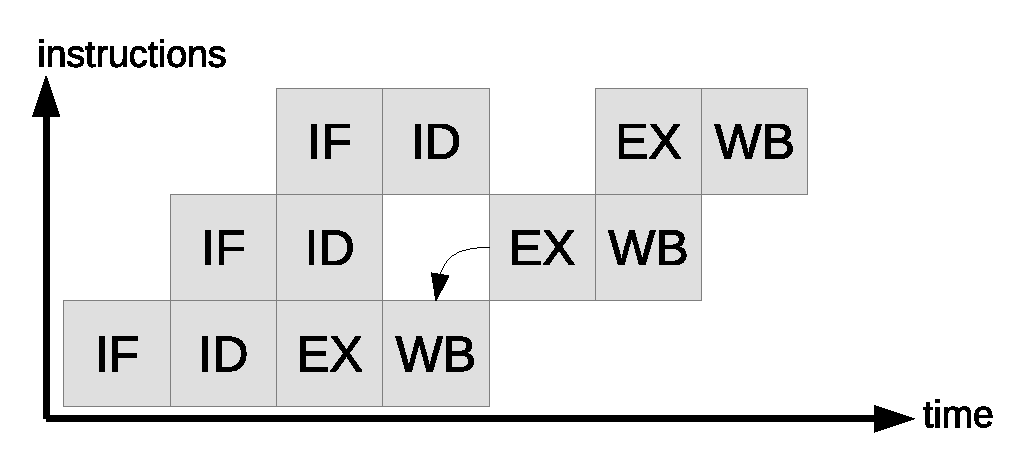
\includegraphics[width=0.5\textwidth]{img/pipeline}
\end{center}
\caption{Model of a filled processor pipeline with a data dependency}
\label{fig:pipeline}
\end{figure}

As most modern microprocessors have multiple execution units for various types of operations (e.g. the x87 floating point unit that's solely purpose is to process floating point calculations), or even have multiple units of the same type, instructions that are executed on different execution unit can be processed in parallel. This is known as \emph{out of order execution}, as the instructions do not necessarily need the same amount of clock cycles and a particular instruction may be outpaced by a succeeding faster instruction, i.e. the instructions are executed ``out of order''. Some modern processors may even reorder instructions on the same execution unit. Out of order execution, just like pipelining, suffers from data dependencies.

In general, data dependencies only measurably diminish performance when appearing in longer sequences (called \emph{dependency chains}), for example in loops. To minimize pipeline stalling, the programmer needs to reduce the number of data dependencies in such loops. Listing~\ref{unrolled} displays an example taken from Agner Fog's optimization manual~\cite[p. 103]{fog2011optimizing}. The increment operation on the loop variable \texttt{i} and the floating point operations are executed on different execution units and thus are likely to be executed out of order. Therefore, the bottleneck is the more expensive floating point addition. In version 1, every floating point addition depends on the result (\texttt{sum}) of the preceding addition, which stalls the pipeline. In constrast, in version 2, two succeeding additions do not depend on each other and thus do not cause a pipeline stall. The technique demonstrated here is known as \emph{loop unrolling}. It usually comes at the expense of additional instructions at the end of the loop (here: \texttt{sum1 += sum2;}), which can almost always be neglected.
\begin{code}[caption={Loop unrolling example}, label=unrolled]
const int size = 100;
float list[size]; int i;

// Version 1:
float sum = 0;
for (i = 0; i < size; i++) 
  sum += list[i];

// Version 2:
float sum1 = 0, sum2 = 0;
for (i = 0; i < size; i += 2) {
  sum1 += list[i];
  sum2 += list[i+1];
}
sum1 += sum2;
\end{code}

%Duffs device?

Another positive effect of loop unrolling is that the loop control branch is evaluated less often. This often leads to better branch prediction results resulting in fewer mispredicted conditional jumps (see Section~\ref{conditional_branches} for further explanation of conditional branches). Apart from loop unrolling, another simple technique to avoid data dependencies and make full use of out of order execution is known as \emph{instruction reordering} or \emph{instruction pairing}. Simply put, instructions that do not depend on each other should be grouped whereas instructions having dependencies between them should be interleaved with other unrelated instructions. For out of order execution it is also desirable to mix instructions which are using different execution units, for example integer and floating point operations. It may not always be easily visible if such measures truly affect the processing inside the CPU, since modern CPUs generally have sophisticated instruction scheduling features and thus ``outsmart'' the programmer. Additionally, performance impact may vary across different CPU generations, for example when newer CPUs contain further execution units. Hence, it is necessary to thoroughly benchmark any optimized code and decide whether these measures are worth the loss of readability, which can be especially bad in the case of instruction reordering.

\subsubsection{Memory performance}
\label{memory_performance}
\paragraph{Stack vs. heap storage of variables.} The memory of an application is divided into two major parts: The stack resides at the beginning of the memory block and is used in a last-in-first-out fashion. When an application allocates a variable on the stack (i.e., all local variables in C), it simply needs to move up the \emph{stack pointer}. The heap usually resides at the end of the memory, growing down. It is used for dynamic memory allocation. When the application wants to allocate memory on the heap, for example because it wants to allocate a dynamically sized array, it needs to ask a heap manager for it (\texttt{malloc} in C). This manager would then look for a storage position that provided sufficient free space for the variable. Managing the heap is much more expensive compared to the simple stack approach, yet it may sometimes be impossible to store all variables on the stack. For instance, in some older programming languages such as C89, it was not allowed to allocate memory on the stack when the size was not known at compile time. Apart from that, the stack is much smaller than the heap and some objects or large arrays may exceed its space limits. However, as the dynamic allocation overhead and additionally the potential memory fragmentation resulting from it reduce performance perceivably, frequently used variables should be stored on the stack whenever possible~\cite[p. 90]{fog2011optimizing}.

\paragraph{Cache misses.} Modern microprocessor architectures feature a multi-level hierarchy of caches which is used to speed up repeated accesses to data values. The Level 1 cache, being the (physically) closest cache available to the CPU, provides the fastest access time. With every successive cache (L2/L3), both access times and cache size increase. For simplicity, I will assume a model of only one cache in the following. Whenever an application uses or manipulates a variable, the CPU checks whether the memory segment where it resides is already loaded into the cache. It if is not, a \emph{cache miss} occurs, resulting in the segment being fetched from main memory. Since the RAM is extremely slow compared to the CPU, the latter is a very time-consuming operation\footnote{In fact, memory access times depend on the internal clockings of the memory modules integrated in the computer as well as the clock frequency of the \emph{Front Side Bus} (FSB), which connects it to the CPU. In ``Principles of Computer Architecture''~\cite[p. 256]{murdocca1999computer} the access time is specified as 60-80 nanoseconds, whereas a register access costs only 1 nanosecond. Although the book is from the late 1990s and the data is likely to be outdated, the proportion should be still valid today.}. The programmer's goal is to reduce the number of cache misses his code produces. The main motivation for today's cache architectures is the so-called \emph{locality of reference} or \emph{data locality}. Basically, data locality refers to probability observations about data access patterns, that are commonly divided into two types: First, temporal locality means that data that has been accessed recently is very likely to be accessed again soon. Second, spatial locality means that data that is spatially close to recently accessed data with regards to its position in the memory (i.e., the memory addresses are similar) is likely to be accessed soon, too. Therefore it makes sense to not only cache a single variable that was recently used, but the whole memory range where this variable resided. Now, to exploit the CPU's caching mechanism, the programmer should adapt his access patterns to these probability estimations. As Agner Fog puts it, ``Variables that are used together should be stored together''~\cite[p. 88]{fog2011optimizing}. This boils down to simple strategies such as always allocating variables when one needs them. As an often used example for cache-friendly variable access, consider the array manipulation in Listing~\ref{seq_array_access}.
\begin{code}[caption={Sequential vs. non-sequential array access}, label=seq_array_access]
int buf[1024 * 1024];

for (int i = 0; i < 1024; i++)
  for (int j = 0; j < 1024; j++)
    buf[i * 1024 + j]++;

for (int i = 0; i < 1024; i++)
  for (int j = 0; j < 1024; j++)
    buf[j * 1024 + i]++;
\end{code}

While both nested loops do the same thing, namely increment each element in the buffer, the crucial difference between them is the way the array index is calculated. While the first loop walks through the array sequentially with the index always growing by one, the second loop ``jumps'' through the array in steps of 1024. The second approach results in a lot more cache misses, as the cache lines get repeatedly displaced by others.

\subsection{Parallelization using Streaming SIMD Extensions}
Created to meet the growing demand for fast multimedia functions in 1996, Intel's MMX technology was the first widely used instruction set extension to deploy the SIMD architecture to modern desktop processors. It used the lower 64 bit of the 80 bit x87 floating point registers to allow for vectorized calculation of 8 bit to 64 bit integers using special SIMD instructions. Its successor, the Streaming SIMD Extensions (SSE), first added 8 separate 128 wide registers for vector calculations (\texttt{xmm0} to \texttt{xmm7}), later complemented by another 8 (\texttt{xmm8} to \texttt{xmm15}) by SSE4. Besides, SSE introduced the possibility to process 4 single or 2 double precision floating point values, on which I will concentrate in the following. Most recently, Intel and AMD have begun to produce new processor lines that include support for the so-called Advanced Vector Extensions (AVX), which can be considered the legal successor of SSE4. The main advantage of AVX over SSE4 is the introduction of 256 bit wide registers and corresponding instructions. Nevertheless, as AVX has only been available on the market for some months and has not changed much with regards to vectorized floating point C code, I will only focus on SSE. The reader may think ``AVX'' whenever I write ``SSE''.

SSE instructions on so-called \emph{packed values} are executed on multiple, physically existing execution units and hence need the same amount of clock cycles as their scalar counterparts. For example, on a 45nm Intel Core 2 processor, both the \texttt{ADDPS} SSE instruction and the \texttt{FADD} instruction have a throughput of 1 instruction per clock cycle~\cite[pp. 50, 57]{fog2011instructiontables}. Whereas \texttt{FADD} calculates the sum of 2 floating point values on the x87 floating point unit (FPU), \texttt{ADDPS} calculates the sums of 4 pairs of floating point values in two \texttt{xmm} registers. Listing~\ref{sse_assembler_intro} shows simplified assembler code that calculates the sum of an array of floats using SSE instructions. Note that this is AT\&T syntax, i.e. source operand before destination operand.
\begin{assembler}[caption={Array sum using simplified SSE assembly}, label=sse_assembler_intro]
  ; ecx contains the length of the array
  ; edx contains the address of the array

  movaps [edx], xmm0
LOOP1:
  add    0x10, edx
  movaps [edx], xmm1
  addps  xmm1, xmm0

  dec    ecx
  jnz    LOOP1

  haddps xmm0, xmm0
  haddps xmm0, xmm0
  movss  xmm0, ebx

  ; now ebx holds the sum of the floats
\end{assembler}

\texttt{movaps} (\texttt{mov}e \texttt{a}ligned \texttt{p}acked \texttt{s}ingle) moves 16 bytes (or 4 single precision floats) between memory and a \texttt{xmm} register. \texttt{addps} adds up 2 registers filled with packed single precision floats vertically. The most interesting part here is the SSE instruction found in lines 13 and 14: \texttt{haddps} horizontally adds adjacent elements in the two operand registers and stores the sums in the destination register, as can be seen in Figure~\ref{fig:haddps}. This illustrates that SSE code usually turns out to be considerably larger in size and number of instructions than scalar code, as the wrapping of data values into vectors (i.e., the ``packing'') and the un-wrapping again are distinct steps that only show up in vectorized code. In this case, the horizontal add would not be needed if the floats were added up one by one.

\begin{figure}[h]
\begin{center}
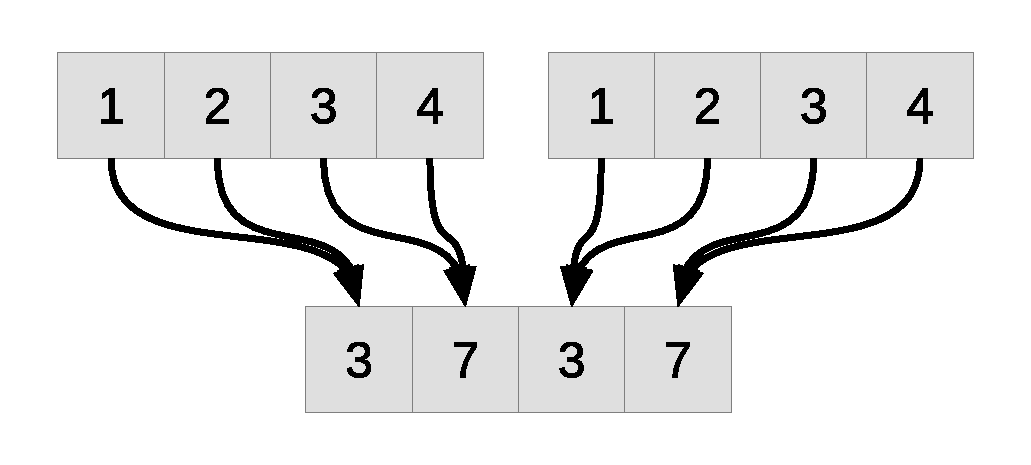
\includegraphics[width=0.5\textwidth]{img/haddps}
\end{center}
\caption{Horizontal Add Packed Single}
\label{fig:haddps}
\end{figure}

The theoretical speed-up factor when enriching scalar code with single precision floating point SSE instructions is limited by the maximum number of floats to be processed simultaneously, which is 4. The mentioned vectorization steps constitute a large enough overhead to easily reduce the speed-up to a factor of 3. However, this speed-up only applies to linear code without control flow statements depending on single data values. Since conditional branches (\texttt{if} statements and the like) inhibit data-parallel execution, they present a difficult to manage obstacle for SSE optimization that needs to be cleared by using special techniques such as blending (see section~\ref{conditional_branches}). These may sometimes impose a performance drawback that completely consumes the expected vectorization speed ups. In practise, my experiments with SSE and moderately complex code resulted in actual speed up factors between 1.5 and 2 (see Section~\ref{Evaluation}).

\subsection{Techniques for programming with SSE}
Fortunately, programming with SSE is well supported by modern compilers. Nowadays, there is no need to use inline assembler at all, as Intel, since the very beginning of MMX and SSE, provided specifications for \emph{compiler intrinsics} for C/C++ languages along the SSE specifications. These intrinsics can be used to instruct the compiler to emit a specific SSE instruction, although the compiler is not obliged to actually comply with the programmer's request. For a start, there were two data types defined that help mixing SSE with legacy code: \texttt{\_\_m128} and \texttt{\_\_m128i}. The former maps to a 128 bit wide floating point vector, the latter a 128 bit wide integer vector. These can be seen as additional primitive data types that behave in the fashion of small fixed length arrays of the corresponding type. Recent versions (>= 4.6) of the GNU compiler collection even let the programmer access single elements using the well-known \texttt{[]}-operator. SSE intrinsic names follow consistent patterns: They all start with a \texttt{\_mm\_} prefix, usually followed by the name of the instruction, followed by the type of the vector's contents. For example, \texttt{\_mm\_hadd\_ps} emits a ``horizontal add packed single'' instruction. It takes two \texttt{\_\_m128} arguments and returns another \texttt{\_\_m128} result value. Listing~\ref{sse_intrinsics_intro} demonstrates the use of SSE instrinsics for the array sum example given above.
\begin{code}[caption={Array sum using SSE instrinsics}, label=sse_intrinsics_intro]
  __m128 sum = _mm_load_ps(&array[0]);
  for(int i = 4; i < count; i += 4) {
    __m128 add = _mm_load_ps(&array[i]);
    sum = _mm_add_ps(sum, add);
  }

  sum = _mm_hadd_ps(sum, sum);
  sum = _mm_hadd_ps(sum, sum);

  // now sum[0] holds the sum of the floats
\end{code}

The GNU compiler collection recently added support for the usual arithmetic operators for vector types, so instead of writing \texttt{sum = \_mm\_add\_ps(sum, add))} we could also write \texttt{sum += add}. This especially helps to minimize readability loss incurred by SSE intrinsics. The use of intrinsics has several advantages over inline assembler. First, as mentioned before, the vector types can be treated as if they were primitives. For instance, the programmer need not to care whether they are stored in registers or in memory. The compiler inserts the appropriate \texttt{mov} instructions when they are needed for calculations. This even includes the possibility to create arrays of vector types. Besides, although almost all SSE instructions use a destructive destination operand (i.e. the second operand of an add operation is also used to store the result), intrinsics will let the compiler copy the necessary register and thus let the programmer reuse his values. Second and even more important, the use of intrinsics leaves some space for compiler optimization. Whether it be register management or the order of instructions, the compiler may always find ways to further optimize the SSE code. In fact, the compiler may choose not to emit a requested instruction at all, if it sees fit. In a blog entry from 2009~\cite{liranuna2009} the author ``LiraNuna'' compares the optimized assemblies of the three major SSE-aware compilers. Apart from revealing considerable differences between the produced assemblies, it also displays that all of the popular compilers were able to further optimize simple SSE intrinsics. For example, gcc succeeded in optimizing out 5 useless vector-based arithmetic operations (e.g. multiplying by a vector whose elements are all 1). In sum, there are rarely any situations where inline assembler has any advantages over the use of SSE intrinsics.

The preparations needed for the code to be of actual practical use are not shown in Listing~\ref{sse_intrinsics_intro}. The array sum would not be correct if count was not a multiple of 4, as then the remaining 1, 2, or 3 elements would not take part in the calculation. There are two options suitable for fixing this issue: Either the programmer could add the remaining elements in a scalar loop right after the vectorized loop (with the iterator starting at the last multiple of 4 less than or equal to count), or he could always pad the array to a length dividable by 4. The padding elements would need to be initialized to zero. Either way would impose a substantial processing overhead (mainly caused by the additional loop) that would render the optimization useless for small arrays. Some other peculiarities of SSE programming are described in the following.

\subsubsection{Aligned data storage} 
Most SSE instructions that operate on either registers or memory locations require those memory locations to be aligned by 16 byte boundaries (in other words, the memory address needs to be dividable by 16). For instance, \texttt{haddps} allows a memory location as source operand, yet will raise a so-called general protection exception when this location is not aligned by 16 bytes, resulting in an application error. For some SSE instructions such as data move instructions (\texttt{movaps}) there exist instruction variants that allow for misaligned addresses (e.g. \texttt{movups}). Shahbahrami et al. discussed the performance impact of misaligned accesses in~\cite{shahbahrami2006misaligned}. The authors point out that, as the processor must rotate or merge registers to support misaligned memory accesses, these accesses will always result in perceptible delays. Besides, misaligned accesses can lead to cache line splits as misaligned memory can be spread over multiple cache lines, which may produce additional slow downs\footnote{In theory, the performance impact of a cache line split should not be any worse than that of an unaligned access. However, an interesting blog entry~\cite{glaser2008cachelinesplits} of x264 developer Jason Garrett-Glaser suggests that cache line splits result in costly penalties on some Intel architectures (e.g., Core 2). Glaser carries on with explaining several SSE-related techniques to circumvent these penalties.}. Their experiments with the addition of two arrays with varying data types and lengths show that aligned accesses using SIMD instructions are on the average about twice as fast as misaligned accesses. The paper also demonstrates various techniques to avoid misaligned accesses.

\begin{figure}[h]
\begin{center}
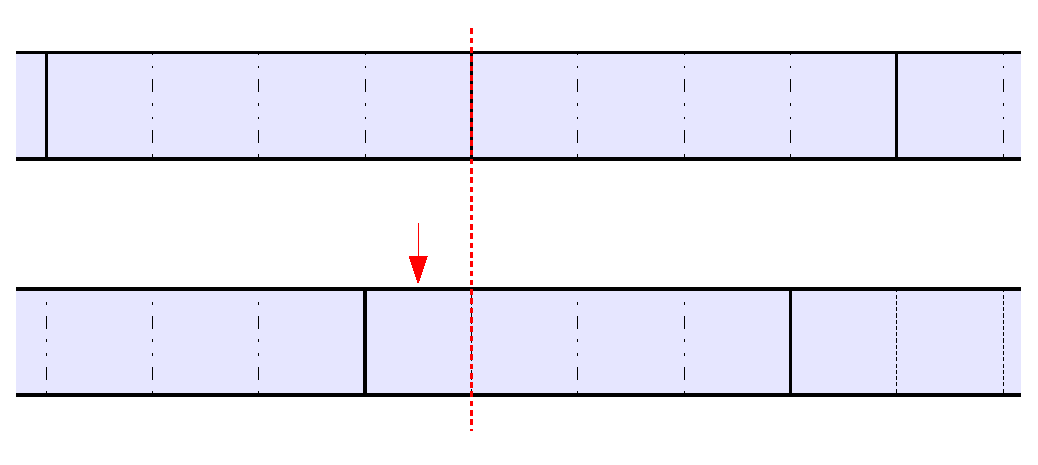
\includegraphics[width=0.5\textwidth]{img/cachelinesplit.eps}
\end{center}
\caption{Example of cache line alignment and cache line split}
\label{fig:cachelinesplit}
\end{figure}

When the programmer can control the allocation of memory himself and the memory should be allocated on the stack, he can easily tell the compiler to align the memory by 16 byte. In gcc this can be done by inserting \texttt{\_\_attribute\_\_ ((aligned(16)))} right after a variable declaration, both for primitives and arrays. The built-in SIMD data types are aligned automatically. Compiler guaranteed alignment of simple data types has the advantage of being totally costless at runtime apart from a possibly increased memory usage. When it is necessary to allocate memory on the heap, the programmer can use special aligning allocators such as \texttt{memalign} or \texttt{valloc} in POSIX compliant operating systems. 

When the programmer has to deal with foreign memory, for example a return buffer from a library call, avoiding misaligned memory accesses will always come with a small processing overhead. When it comes to iterativly processing such a misaligned array, the obvious and probably most practical approach is called \emph{loop peeling} or \emph{loop splitting}. Here, the relevant loop is split up into three parts: the main loop, in which the bulk of the array is processed using SSE instructions, is framed by two loops containing scalar code to process all elements before the first and after the last 16 byte boundary in the array. See Listing~\ref{loop_peeling} for an example. Yet, these additional loops (especially their conditional jumps) amount to increased processing time that can effectivly consume the expected performance gains in some situations. Another simple approach useful for situations with small data that gets created once but is read often would be to copy the data to an aligned memory address.

\begin{code}[caption={Loop peeling example}, label=loop_peeling]
  // Iterate to the first memory address dividable by 16.
  float sum = 0;
  int i = 0;
  for(; (i < count) && (&array[i] % 16 != 0); i++)
    sum += array[i];

  // Vectorized main loop.
  __m128 tmp = _mm_load_ps(&array[2]);
  for(; i < count - (4 - i); i += 4) {
    tmp += _mm_load_ps(&array[i]);
  }
  tmp = _mm_hadd_ps(tmp, tmp);
  tmp = _mm_hadd_ps(tmp, tmp);
  sum += tmp;

  // Add remaining elements.
  for(; i < count; i++)
    sum += array[i];
\end{code}

\subsubsection{Dealing with conditional branches}
\label{conditional_branches} 
The by far hardest hurdle in SSE programming is the transcription of conditional branches. Conditional jumps depending on single values obviously can not exist in data-parallel code and thus need to be replaced by some arithmetic or logical linear statements. For example, consider that we wanted to sum up only those elements of the float vector (refer to Listing~\ref{sse_intrinsics_intro}) that are greater than 5. In a scalar version this would require an \texttt{if} statement within the \texttt{for} loop that, when evaluated to \texttt{true}, would allow the current float to be added to the sum. Getting rid of the conditional jump in scalar C code is possible through evaluating the logical value of a comparison as an integer. Knowing that \texttt{false} is defined to be an integral zero and that \texttt{true} is equal to 1 in most C implementations, we could replace the \texttt{if} statement and therefore the conditional jump with: \texttt{sum += array[i] * (array[i] > 5)}. Comparisons in SSE also define zero as the value of \texttt{false}, but return \texttt{-NaN} as \texttt{true}, which translates to negative ``Not A Number'' or 0xFFFFFFFF, a bitmask that has a 1 at all positions. Thus, whereas scalar C code requires a multiplication to eliminate the conditional jump, SSE takes a bitwise conjunction. See Listing~\ref{sse_blending_intro} for a SSE implementation that calculates the sum of all array elements which are greater than 5.

\begin{code}[caption={Sum of array elements greater than 5}, label=sse_blending_intro]
  __m128 sum = _mm_setzero_ps();
  __m128 five = _mm_set1_ps(5.0f); // (5.0, 5.0, 5.0, 5.0)
  for(int i = 0; i < count; i += 4) {
    __m128 add = _mm_load_ps(&array[i]); // e.g. (1.0, 6.0, 2.0, 8.0)
    __m128 mask = _mm_cmpgt_ps(add, five); // -> (0.0, -NaN, 0.0, -NaN)
    sum += _mm_and_ps(add, mask); // -> (0.0, 6.0, 0.0, 8.0)
  }
\end{code}

If the conditional had an \texttt{else} branch containing a different assignment statement, the SSE code would require two additional bitwise logical operations, namely an \texttt{ANDNOT} for the \texttt{else} assignment and an \texttt{OR} to blend the results of the branches. With SSE4, this triple of bitwise operations has been compacted into a single instruction called \texttt{blendv} (along with other types of blending operations) that merges the bits of two vectors based on a third mask vector. 

In general, performances of vectorized code sections that work around conditionals largely depend on two factors: Probabilities of truth values and the amount of computation done in the related branches. For simple branches such as the assignment statement above it is usually true that a vectorized solution will outperform the scalar version as conditional jumps have a significant impact on performance. Whenever a conditional jump appears in application code, the processor tries to guess what path will be taken and precalculates that branch's results. When the guess turns out to be wrong (\emph{branch misprediction}), the precalculation needs to be discarded and the processor's pipeline needs to be flushed, which can easily stall the processor for a hundred clock cycles. In contrast, vectorized code always evaluates both possible branches and blends the result according to a conditional bitmask, as explained above. As there are no conditional jumps, branch mispredictions become irrelevant. Yet, modern processors feature advanced branch prediction technology and often branch mispredictions get fairly uncommon. In some cases, this may even get to the point where a well predictable condition that determines whether a larger amount of code will be executed or not turns out to be faster than the corresponding vectorized code without condition that will always execute that code. As an extreme example, consider a basic \texttt{if} clause that evaluates to \texttt{true} only once in a thousand runs but then will lead to a considerable portion of code. Here, scalar code may turn out to surpass the performance of its vectorized counterpart. This issue also takes effect in long loops that contain ``early out'' conditionals (e.g. an early \texttt{if}-\texttt{break} group), since the loop needs to be executed until that conditional is \texttt{true} for all vector elements, when it may have canceled the loop for single elements much earlier.

When dealing with long code sections guarded by a conditional, the straightforward approach is to blacklist vector elements that should not take part in the calculation in a blacklist vector. Statements that have no outside effects can then be executed for the whole vector, while those that have outside effects need to be blended depending on the blacklist or need to be performed during or after the unwrapping of the vectors. It may also be possible to omit the blacklist vector and instead directly incorporate the \texttt{NaN} value resulting from the comparison into the calculation. Any operation including a \texttt{NaN} value will always return another \texttt{NaN} value, so the initial \texttt{false} from the comparison will show up at the end of the calculation. However, this may only lead to a small speed-up in comparison to an explicit blacklist vector, mostly due to the blacklist likely having been dropped from cache. Occasionally it may even be feasible to omit the comparison, if the succeeding instructions will always lead to zero or infinity values for those vector elements that originally would have been sorted out by the comparison. However, as this is an arithmetic optimization, it might as well have been done in the original scalar code in the first place.

In case a conditional frequently evaluates to \texttt{false} for all vector elements, the new SSE4 \texttt{ptest} instruction comes to help. This instruction is especially valuable for the above mentioned case of rarely executed code sections after a conditional that is unlikely to be \texttt{true} at all. \texttt{ptest} is the first SSE instruction to operate on the 128 bit value as a whole, it does a bitwise comparison of two \texttt{xmm} registers and returns a scalar \texttt{true} or \texttt{false}. Additionally, Intel provided some helpful convenience intrinsics that test a vector for ``all 1'' or ``all 0'' values which are named \texttt{\_mm\_test\_all\_zeros} and \texttt{\_mm\_test\_all\_ones}. See Listing~\ref{ptest} for two examples of \texttt{ptest} usage.

\begin{code}[caption={Examples of \texttt{ptest} usage},label=ptest]
// Rarely true condition.
__m128 cmp = _mm_cmpgt_ps(a, b);
if(! _mm_test_all_zeros(cmp)) {
  // Rarely executed code.
}

// Test whole vectors for equality.
// Cast intrinsincs do not actually emit an instruction,
// but instead only statically cast the vector types.
int equal = _mm_testc_si128(_mm_castps_si128(a), _mm_castps_si128(b));
\end{code}

\subsubsection{Prefetching \& non-temporal streaming}

When trying to optimize memory throughput of an application, the programmer can manually control cache management with prefetching and streaming. Prefetching, on the one hand, instructs the processor to preload memory into the caches that will be needed soon. This, however, rarely has any effect on performance as modern processors integrate fairly optimized hardware prefetching technology. Yet, in some cases it may yield some improvements when used in the right way. Manual prefetch instructions should always point far ahead in memory (e.g. 500 bytes) and should only be issued when the programmer is absolutely confident that he will need the memory soon and that it has not been cached already. Also he needs to make sure that prefetching does not displace already cached memory segments that are going to be used prior to the prefetched memory, which would result in a performance decline. This is commonly refered to as ``cache thrashing'' and may be considered a rare worst case scenario. Note, that the prefetch instruction is only a hint to the processor which it may or may not obey, in fact, the instruction may not do anything at all, when the processor already is busy loading different segments of memory. Prefetching will always require a fair bit of trial and error and in my experiments resulted in virtually zero performance improvements.

Streaming, on the other hand, is a rather common technique that can significantly increase memory throughput. The \texttt{movnt--} family of SSE instructions (e.g. \texttt{movntps}, meaning ``move non-temporal packed single'') hint the processor that the data that should be moved to memory will not be needed again soon. ``non-temporal'' relates to the temporal characteristic of the before mentioned ``reference of data'' (again, refer to Section~\ref{memory_performance}) which is the foundation of today's cache architecture. When the processor encounters a \texttt{movntps} instruction, it will try to write the data directly to memory and bypass its caches. This has two major advantages over the regular move instructions: First, it is not necessary to read the memory segment to cache first, which results in a noticeable speed-ups if the memory segment has not been loaded to cache already. Second, it will avoid polluting a cache line with pointless data, so that data that may be used again can remain in cache. Though, non-temporal data moves will only avoid caching when used with data big enough to fill up an entire cache line, i.e. at least 64 bytes on most systems. This is due to the fact the processor can only bypass the cache if it is able to use its ``write-combining'' buffers. Apart from that, a common advice seems to be to issue a \texttt{mfence} instruction following the non-temporal streaming instructions, which stalls the processor until any memory operation has completed, in order to ensure that succeeding reads from that memory return the correct data. AMD has provided a helpful summary of how to properly use streaming instructions in their optimization manual~\cite[pp. 106ff, 231ff]{amd2012optimization}. Since SSE has become an industry standard that both Intel and AMD are committed to fully support, most of the information presented in this manual should apply to Intel processors as well.

In order to experience the speed-up of streaming store instructions myself, I wrote three different \texttt{memset} implementations for floating point values. Table~\ref{memset_table} displays results of these experiments using different compiler optimization options (from \texttt{-O0} to \texttt{-O3}). As can be seen easily, the SSE implementation based on simple store instructions turns out to have no impact on performance at all with compiler optimization is turned on, which is likely due to the compiler having auto-vectorized the loop in the scalar version. Streaming store instructions, in constrast, outperform the other implementations by factor 2. It seems impossible for the compiler to determine if the data written to memory is going to be reused soon, thus it does not emit streaming store instructions itself. The code of this benchmark can be found in Appendix~\ref{memset_code}.

\begin{table}[h]
\begin{center}
\caption{Comparison of \texttt{memset} implementations}
\begin{tabular}{lcccc}
\toprule
Implementation & Runtime (s), -O0 & -O1 & -O2 & -O3 \\
\midrule
scalar memset & 0.179 & 0.999 & 0.993 & 0.0987 \\
SSE memset (\texttt{mov} instructions) & 0.100 & 0.102 & 0.103 & 0.100 \\
SSE memset (\texttt{movnt} instructions) & 0.069 & 0.041 & 0.039 & 0.039 \\
\bottomrule
\end{tabular}
\label{memset_table}
\end{center}
\end{table}

\subsection{A word on compiler optimization}
Whenever a programmer chooses to optimize a particular piece of code, he has to be aware of the fact that the compiler --- when used with the right set of command line arguments --- usually may have already created optimal machine code from that code. As a consequence manual code optimization very often will not yield the desired performance improvements but instead may even slow down the application. Besides, manual optimization will always be a time-consuming task and in the end lead to less readable code. Felix von Leitner gave a striking speech~\cite{leitner2009} about compiler optimization at ``Linux Kongress'' conference 2009 in which he emphasizes that it is far more important to learn how compiler optimization works and how to structure code in a way that supports compiler optimization than to try to manually outperform the compiler. He concludes that only when the performance boost ``drastically'' outweighs the decrease in readability, manual optimization really is worth the effort. Again, I would like to point out that the value of manual optimization depends on the very situation. Although on a small scale the compiler will most of the time create fast enough code and manual optimization may not improve performance at all, a human programmer may find optimization measures at a larger scale that speed up execution a lot. The same is true for vectorization: Most modern compilers are able to auto-vectorize specific parts of code such as smaller loops without data dependencies. However, compilers are not able to grasp the complexity of longer loops that could be vectorized as well, for example using branch avoidance techniques as described above.
\section{Optimizing the LS$^{2}$ simulation engine}
\label{Implementation}
In the following section I will describe how I optimized the LS$^{2}$ simulation engine using mainly SSE intrinsics. I will begin introducing the software itself and its research purpose. Then, I will document the approach taken for development, including information about how I benchmarked the application in order to acquire meaningful results. The main part of this section will be comprised of a detailed explanation of the optimized source code of the three algorithms that I have chosen to improve.
\subsection{LS$^{2}$: A simulation engine for lateration algorithms}

The term "lateration algorithms" is commonly used to refer to geometric algorithms that use distance measurements to determine the location of points in the plane or in a three-dimensional space (as opposed to triangulation which uses the measurement of angles). The most basic representative of this group of algorithms is known as \emph{trilateration}: Obviously, in the euclidean plane it needs at least three known spots (subsequently called \emph{anchors}) and the distance measurements hereof to be able to narrow down the current position to a single point. Relative to each of the anchors, this point lies on a circle that has its center on the anchor and the distance as its radius. Trilateration determines the current position by solving these three linear equations, in other words, it calculates the intersection of the three circles drawn around the anchors. In real-world applications such as the Global Positioning System (GPS) or indoor localization, distance measurements, like all physically measured data, are generally error-prone. Most commonly, distances are estimated by measuring the time it takes a signal (e.g. light, radio) to travel between an anchor and the client. Because of these erroneous distances, circles drawn around the anchors do not necessarily intersect at a single point and the basic trilateration algorithm fails to produce an exact result. In order to calculate an approximation of the current position, trilateration can be adapted to return the geometric center of the now up to three circle intersections. However, during the last decades, several superior, more complex algorithms have been found that compute improved position estimations based on error-prone distances of three or more anchors.

The \emph{FU Berlin Parallel Lateration-Algorithm Simulation and Visualization Engine} (LS$^{2}$), written by Heiko Will, Thomas Hillebrandt, and Marcel Kyas and first presented at the WPNC conference 2012, is a graphical evaluation framework for lateration algorithms. As the authors explain in~\cite{will2012ls2}, the application's fundamental idea is to not only calculate an average algorithm error based on randomized locations, which has been the main evaluation criterium for lateration algorithms so far, but to calculate errors for all locations on a given "playing field" in parallel and in the end to provide the user with an image displaying the so-called \emph{spatial position error distribution}. The assumption is that the position of the anchors has significant influence on the algorithm's performance, even more so than the errors of the distances. Figure \ref{fig:lateration} shows an exemplary output image created with the LS$^{2}$ engine using the "vble\_opt" algorithm and a set of 3 anchors, only the anchor positions have been slighty magnified for better visibility. The left part of the image displays the average position error for every location (where yellow means low average error), whereas part to the right displays the highest error for every position.

\begin{figure}[h]
\begin{center}
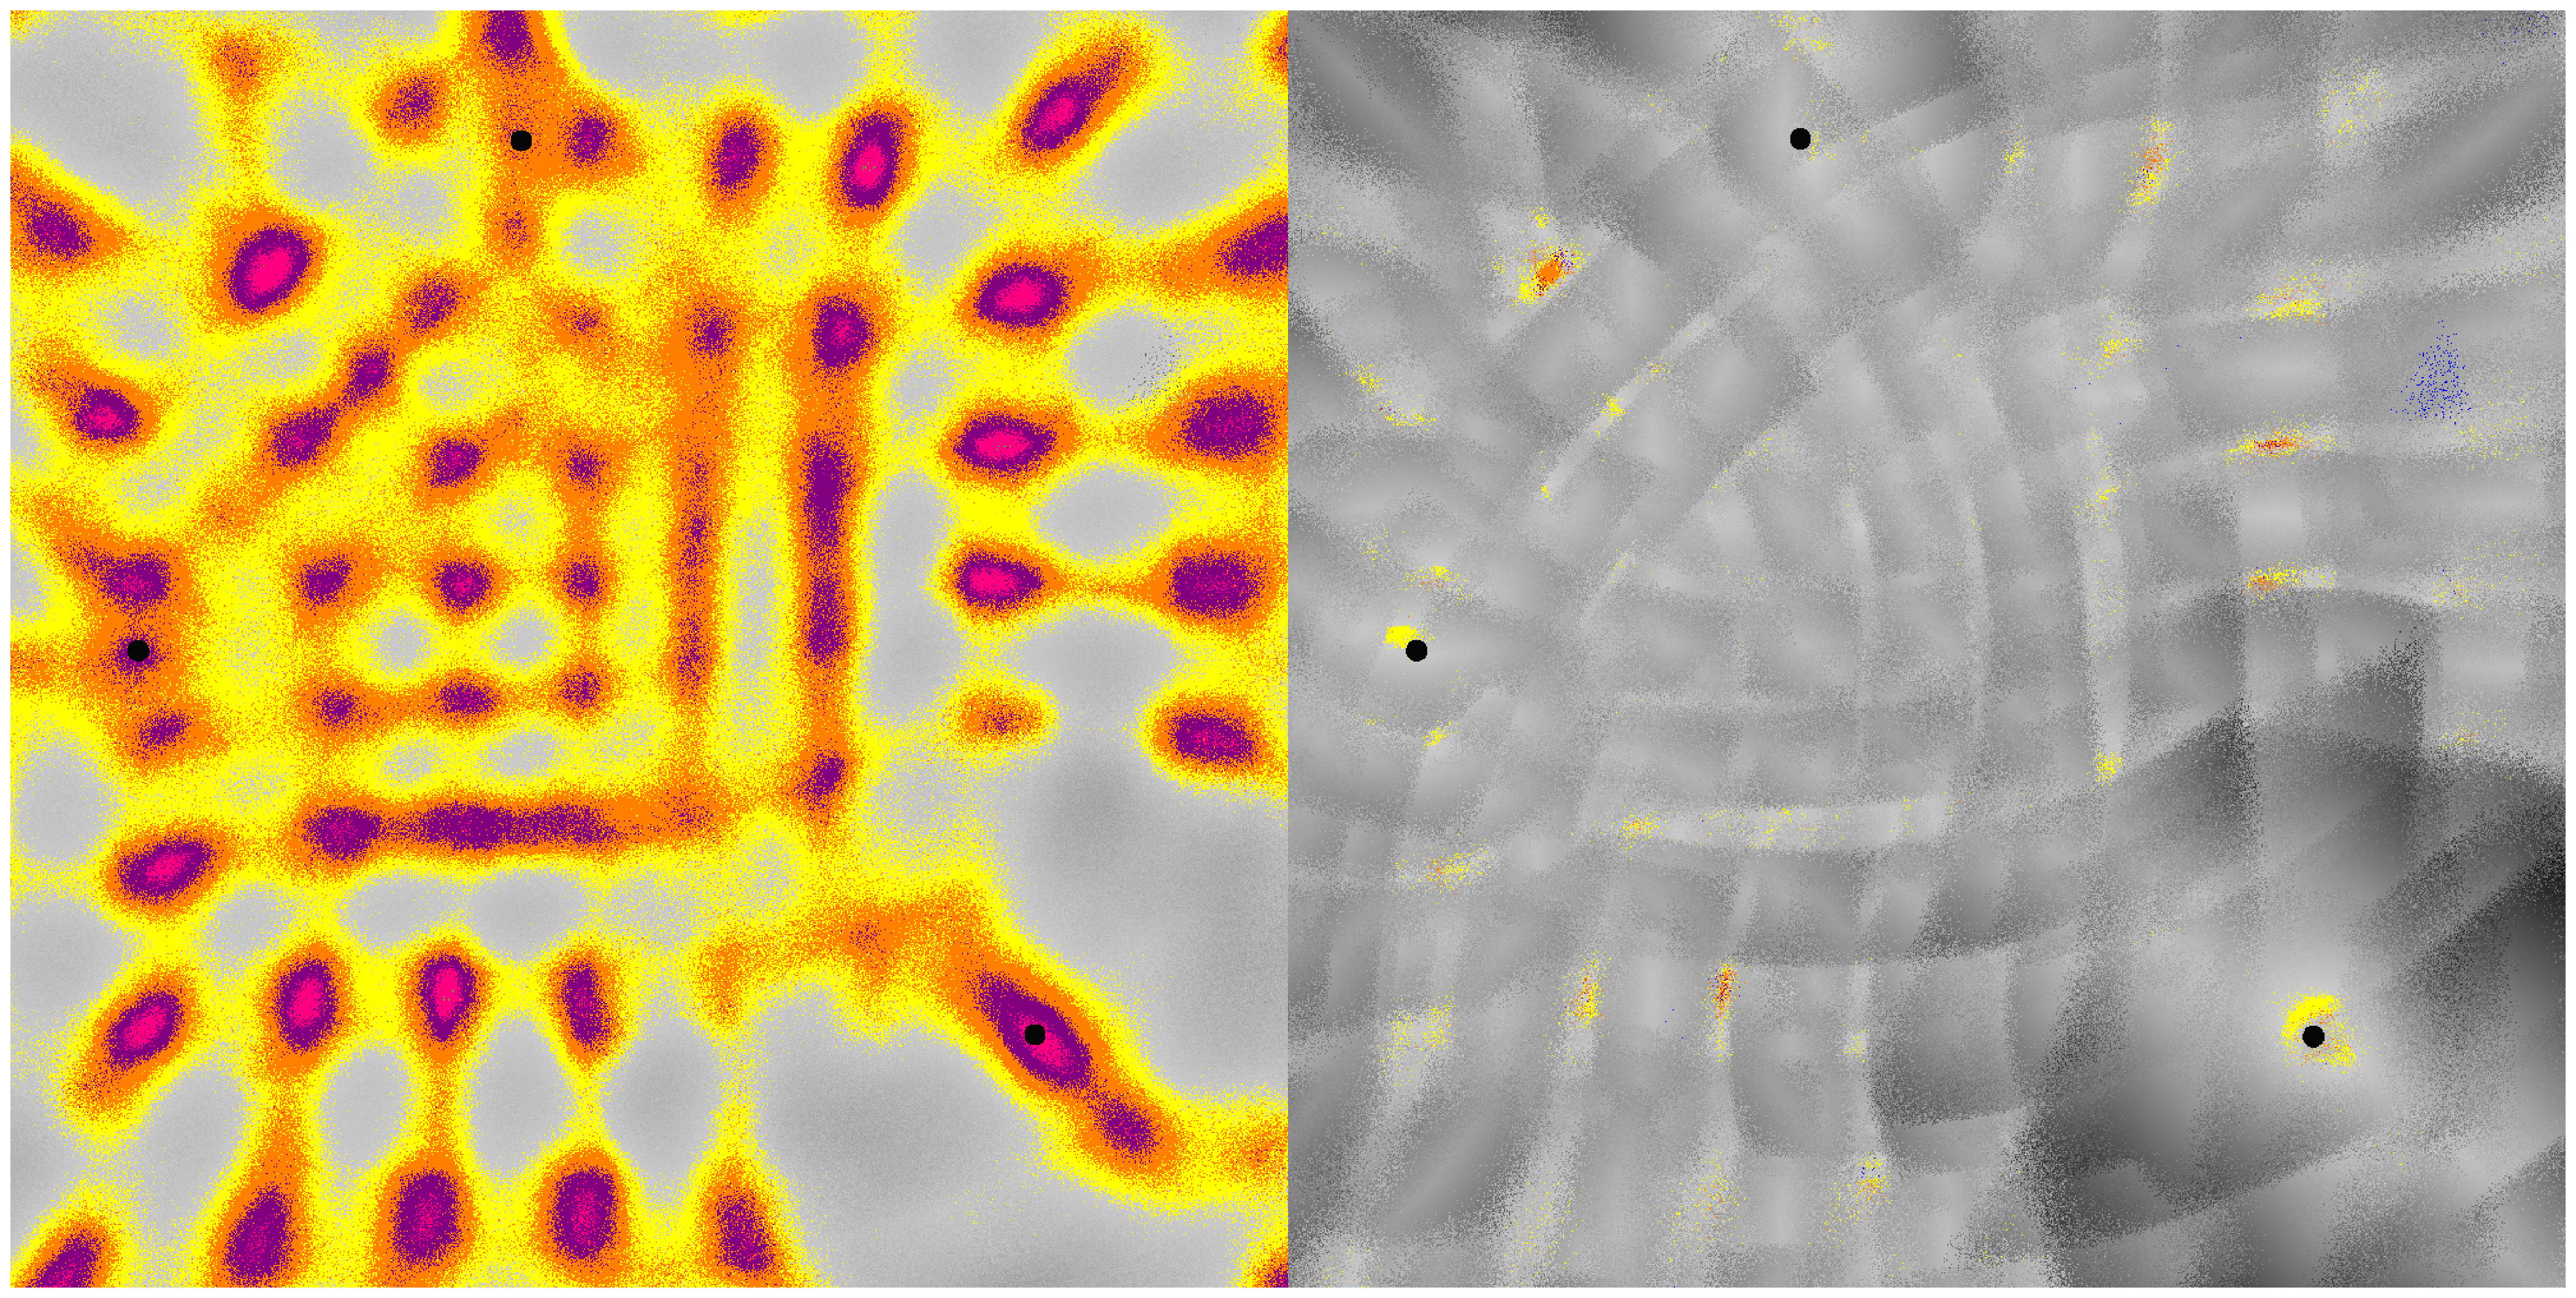
\includegraphics[width=14cm]{img/lateration}
\end{center}
\caption{Example output of the LS$^{2}$ engine}
\label{fig:lateration}
\end{figure}

The application is divided into three main parts: The engine itself, responsible for distributing the work load and calculating the position errors, a set of error models, which are used to simulate the distance measurement errors, and the lateration algorithms. Parametrized with a set of anchor positions, the error model, and the desired algorithm, the engine first starts a number of threads and associates them with a spatial slice of the 1000x1000 playing field. For each position in its slice, a thread calculates the real distance between the position and the anchors, randomly modifies the distances according to the error model, and executes the lateration algorithm. It then calculates the algorithm error as the difference between the real distance and the algorithm's return value. This process is repeated for a configurable number of iterations (defaults to 40) for each position, before the resulting average error is written back to an image buffer. At the time of writing, LS$^{2}$ features 6 different lateration algorithms, of which 4 are standard algorithms such as trilateration or adapted multilateration (AML) and 2 are novel algorithms provided by the authors themselves. Regarding the error model, the user can choose between a uniform distribution and a Gaussian distribution of error values, although work is underway to support map-based error models as well.

The LS$^{2}$ engine is implemented in C99 dialect and is heavily optimized for speed. All functions are forcibly inlined and reside in the same compilation unit. Apart from the image buffer, no dynamically allocated memory is used. The engine itself uses SSE instructions or, at the user's wish, the newer AVX instructions available on Intel's most recent Sandy Bridge microprocessors, to process 4 respectivly 8 iterations at once. For example, the calculation of the true distances is fully vectorized as is the random number generator used by the error models. Afterwards, the engine will execute the user-requested lateration algorithm with vectorized parameters. To understand the mechanics, refer to listing \ref{prototype} which shows the function definition of the trilateration algorithm. The \texttt{count} parameter specifies the number of anchors the algorithm should use, whose x- and y-coordinates are contained in the \texttt{vx} and \texttt{vy} arrays. Note, that these, as well as the distance array \texttt{r} and the result buffers \texttt{resx} and \texttt{resy}, are declared as \texttt{VECTOR}s, which means that there are 4 (resp. 8) of each of these values waiting to be processed at once.

\begin{code}[caption={Prototype of the \texttt{trilaterate} function},label=prototype]
void trilaterate(const int count, const VECTOR* vx, 
                 const VECTOR* vy, const VECTOR* r, 
                 VECTOR* resx, VECTOR* resy);
\end{code}

When I started looking into optimizing the LS$^{2}$ application for this thesis, some algorithms shipped with it, for example trilateration and \texttt{lin\_lsq} ("Linear Least Squares"), already made use of SSE instructions to process their parameters in a single run. Yet, some others were merely literal transcriptions from a scalar implementation and were not aware of vector processing at all. These algorithms (\texttt{geolat}, \texttt{vble\_opt}, and \texttt{aml}) simply unwrapped the vectors at the function head, calculated the position estimations in scalar code, and packed the results back into the result buffers at the end of the function. Therefore, these three algorithms best qualified for having a deeper look into their optimization potential.

\subsection{Development approach}
During the development period, it quickly became clear to me that software optimization is not an utterly straightforward task, but instead is a rather non-linear process involving mostly trial and error methods. Quite often attempting to optimize a particular piece of code using a specific optimization technique would not lead to any performance gains, even though in theory it may have looked like a very promising measure. Yet sometimes, these attempts that seemed to be "dead-ends" at first try later became valuable complements to other optimization efforts. As a consequence, my "development process", which was anything but well-defined at the beginning, turned out to be slightly different from regular iterative processes. As it is mainly a report on my personal experiences, the following section should not be misinterpreted as a universal guideline. The described steps and tools simply suited my needs best, but may seem completely pointless for others.

\subsubsection{Determining bottlenecks through profiling}
As Donald E. Knuth has already stated memorably in 1974, it is a good idea to first determine the most performance-critical part of a piece of code before beginning with optimization work, as this is likely the only part where optimization really is worth the effort. To find that critical part, the performance bottleneck, profiling a software can be helpful. For C/C++ code and Unix-like platforms, a tool called \emph{Valgrind}\footnote{\url{http://valgrind.org}, last accessed: \today{}} has become the de-facto standard profiler utility. The Valgrind suite consists of a variety of specialized profiling tools, each of them named differently, as for instance a memory usage analyzer (Mmemcheck) that especially helps finding memory leaks, a heap profiler (Massif) for dynamic memory profiling, and a cache profiler (Cachegrind) that simulates cache utilizitation to detect cache misses. The latter is especially valuable for optimization, as it additionally counts the executed instructions for each code line and is able to estimate the amount of clock cycles the processor needs to execute them. On top of that, Cachegrind features a special option (\texttt{--branch-sim=yes}) that counts branch mispredictions and thus can identify particularly unpredictable branches. Cachegrind's result can be best viewed using the \emph{KCachegrind}\footnote{\url{http://kcachegrind.sourceforge.net/html/Home.html}, last accessed: \today{}} front-end, as demonstrated by the screenshot in figure \ref{fig:kcachegrind}.
\begin{figure}[h]
\begin{center}
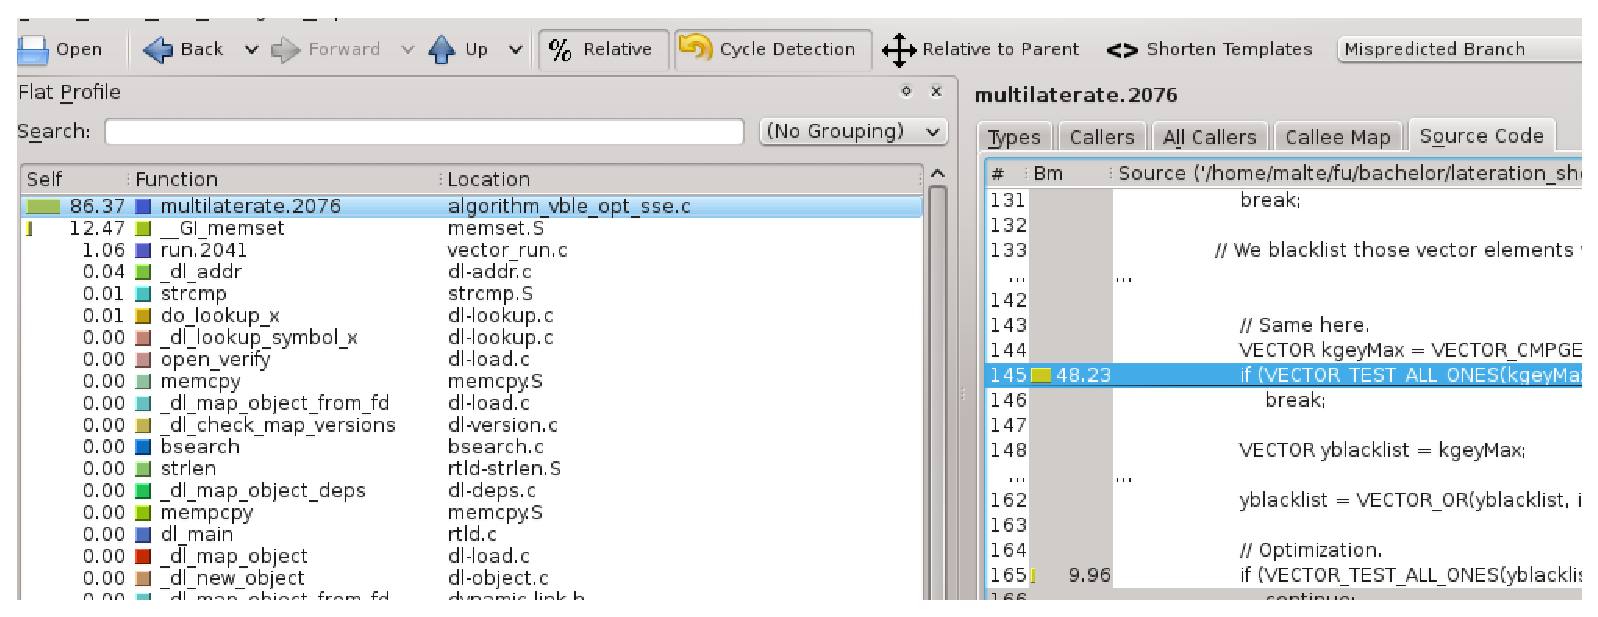
\includegraphics[width=14cm]{img/kcachegrind}
\end{center}
\caption{KCachegrind displaying branch mispredictions}
\label{fig:kcachegrind}
\end{figure}

\subsubsection{Benchmarking optimization efforts}
After having identified the bottlenecks and resolved them with the help of optimization techniques, the next step is to evaluate their impact on performance. Before and after every smaller step, I used the unix \texttt{time} command to measure performance of the application for a randomly selected set of input values. As can be read on the command's manpage, \texttt{time} measures three different execution times, see listing \ref{time} for an example output. The "user" value indicates the amount of CPU time spent in user-mode, the "sys" value is the amount of CPU time spent in kernel-mode. The "real" value is the real time that has elapsed between start and termination of the application. For threaded applications such as LS$^{2}$, on dual-core systems this should ideally be about half of the combined "user" and "sys" times plus some overhead for context switches. As the "real" time varies with the number of processors available and the number of system-calls contained in LS$^{2}$ is close to zero, the only information that made a difference for my optimization work was the "user" value.
-
\begin{shell}[caption="Example output of the unix \texttt{time} command",label=time]
$ time { ./bin/lateration_shooter_sse 100 400 500 200 700 800 ; }
Average error is 45.252751

real    0m8.056s
user    0m14.916s
sys     0m0.008s
\end{shell}

As the performance of the various algorithms in LS$^{2}$ turned out to be highly affected by the positions of the anchors, it was also crucial to evaluate the performance gains using a larger amount of randomized input data, in order to avoid optimizing the application for a single case. For this time-consuming task I wrote an increasingly useful Python script dubbed \emph{benchlat}, which compiled my various work states, executed them a ĺarger number of times overnight, and after completion sent me an email containing the analyzed results, namely average and variance of the runtimes. Later I added automatic profiling using Cachegrind as well as an option that allowed tracing the performance fluctuation through the development history. Regarding the selection of anchor positions, I decided to mainly choose points close to (distinct) borders of the playing field. This reduces the bias towards small, centered shapes that would arise from a uniform distribution of points and in general can be considered more realistic for localization scenarios [THIS SCREAMS CITATION.]. In order to provide statistically reliable data, benchlat empirically detected the convergence of the runtime average (after an initial threshold of 100 runs), with the convergence criterion defined as, "average has not oscillated more than $\pm0.001$s within the last 10 runs". All benchmark results displayed in the following sections have been produced by benchlat.

\subsubsection{Managing various attempts using a version control system}
As mentioned before, optimizing LS$^{2}$ was an unsteady task that was characterized by hours of trial and error. When an optimization proved to be the best solution in the very situation and to measurably improve performance, I integrated it into the sources and moved on to the next chokepoint. These successes were often preceded by a number of less profitable attempts that I wanted to save for possible later reuse. Making heavy use of lightweight branches as provided by most modern version control systems such as Git\footnote{\url{http://git-scm.com/}, last accessed: \today{}} proved highly beneficial for these cases. Using branches, I could temporarily put unpromising changes aside and merge them back in when they again seemed attractive solutions in combination with other work. To illustrate the trial and error process more vividly, figure \ref{fig:branchtree} displays a schematic overview of the development in form of a visualization of the complete Git history. Nodes represent the numerous Git commits, which are linked by arrows indicating an "ancestor-of" relationship. As can be easily seen, the development path was by no means a straightforward one.

\begin{figure}[h]
\begin{center}
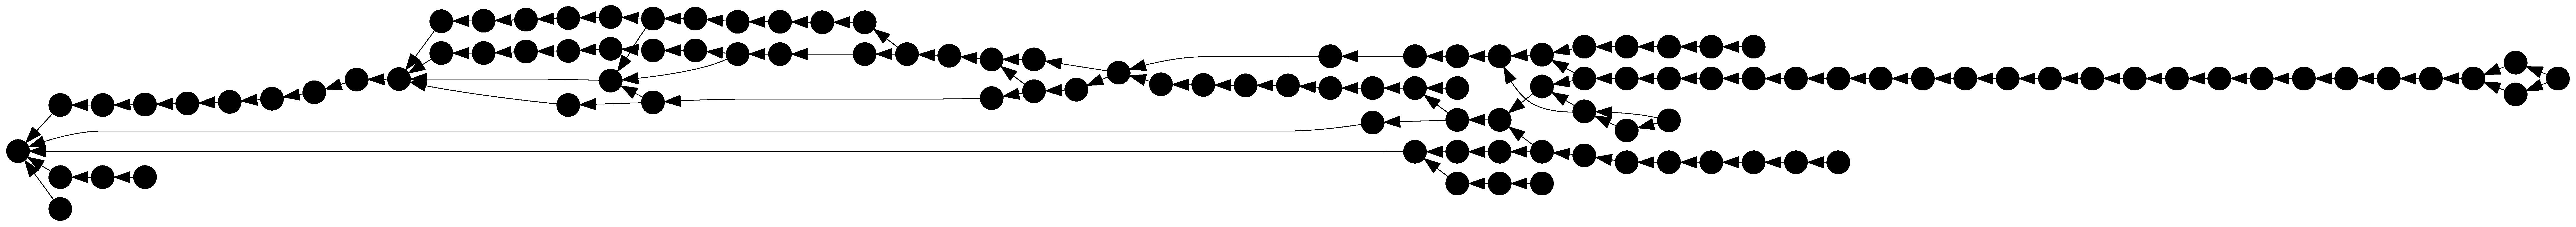
\includegraphics[width=14cm]{img/branchtree}
\end{center}
\caption{Visualization of \texttt{git} history}
\label{fig:branchtree}
\end{figure}
\subsection{Algorithm I: aml}
\subsubsection{Introduction}

\subsubsection{Optimizations}
\subsection{Algorithm II: geolat}
\subsection{Algorithm III: vble\_opt}
\subsection{Framework}
--> movntps yyx
\subsection{Evaluation}
\label{Evaluation}

In the following, I will evaluate the outcome of my optimizational work. Using experimental benchmark data, I will discuss the impact of the optimizations on the three algorithms and reason about the influence of anchor positions on each algorithm's performance. I will also debate the statistical significance of these benchmarks.

\subsubsection{Approach}
\label{eval_approach}
As mentioned in Section~\ref{benchmarking}, the following data has been collected using my custom-made \emph{benchlat} utility. For this final benchmark, the algorithms were executed 500 times each, using 3, 4, and 5 anchors for AML and VBLE-OPT, and only 3 anchors for Geo3, which simply discards additional anchors. Regarding the selection of anchor positions, I decided to mainly choose points close to distinct borders of the playing field, aiming at a near uniform distribution of the area of the shapes formed by the anchors, and at avoiding having a bias towards small, centered shapes that would arise from a uniform distribution of points. This can in general be considered more realistic for localization scenarios. Though, since the input parameters are discretized to integer simulation units by the engine, this constraint also resulted in a lower bound on the area of the anchor shape. For example, one minimal triangle would be formed by three points lying as close as possible to one border of the playing area without being colinear, for example, the points (1|0), (0|500), and (1|1000). This triangle still has an area of 500 square simulation units.

After each algorithm's run, the original implementation of the algorithm was executed using the same set of anchors, in order to obtain a reference runtime. Both the reference and the optimized runtimes were reduced by the constant overhead imposed by the engine itself, which is mainly composed by the time it takes the engine to calculate the real distances and to generate the random measuring errors. In order to estimate this overhead, I executed the \emph{const} algorithm shipped with LS$^{2}$, which does nothing but return the input parameters, a thousand times and calculated the average of the runtimes. The resulting average overhead is 0.06603 seconds. 

The achieved speed-up of each anchor and algorithm combination was calculated using Formula 1 shown below, where $t_{o,i}$ denotes the optimized runtime and $t_{r,i}$ is the reference runtime. The average speed-up was derived using the usual formula for the arithmetic mean that is displayed in Formula 2.

\begin{align}
s_{i}& = \frac{t_{r,i}}{t_{o,i}} \\
\texttt{average}& = \frac{1}{n} \cdot \sum_{i = 1}^n s_{i}
\end{align}

The benchmarks were run on a quad-core Intel Xeon E31245 CPU with a clock frequency of 3.30~GHz, which had access to a total of 8~GB main memory. Because availability of this system was temporally limited, the number of algorithm iterations for each position needed to be reduced to 40, though, as execution runtimes are linearly dependent on the number of iterations (refer to Section~\ref{ls2}, this does not compromise the significance of the benchmark results. The framework was configured to always use uniformly distributed errors. This, by contrast, limits the universality of the benchmark results to some degree. However, at the time of my coding it was the only error model implemented in LS$^{2}$. The application was compiled using the GNU compiler collection, version 4.6.3, with compiler optimization set to \texttt{-O3}.

\subsubsection{Discussion}
To begin with, all benchmark runs have delivered a positive result, i.e., the performance of each algorithm has been improved no matter where the anchors were placed. Table~\ref{average_table} shows the average speed-up calculated over all benchmark runs for each algorithm for 3, 4, and 5 anchors, providing a convenient overview of how much the algorithms benefitted from the optimization. AML boasts the best results with an average speed-up of 2.7 to 3.0, followed by Geolateration and VBLE-OPT.

\begin{table}[ht]
\begin{center}
\caption{Average speed-ups}
\begin{tabular}{lccc} 
\toprule
& \multicolumn{3}{c}{Average speed-up} \\ 
\cmidrule(r){2-4}
Algorithm & 3 anchors & 4 anchors & 5 anchors \\
\midrule
AML & 3.30 & 3.34 & 3.36 \\
GEO3 & 2.20 & N/A & N/A \\ 
VBLE-OPT & 1.68 & 1.77& 1.75 \\
\bottomrule
\end{tabular}
\label{average_table}
\end{center}
\end{table}

Most prominently, the AML speed-ups seem to increase linearly, which was affirmed by (less numerous) experiments I conducted with 6 to 8 anchors. This is likely caused by the growing influence of the \emph{refinement} step, that could be perfectly vectorized due to the absence of conditional statements and thus has a considerable advantage over the scalar implementation. Using fewer anchors, the \emph{first intersection} step becomes the prevalent factor limiting the overall performance. However, as mentioned in the introduction, the theoretical speed-up of a SSE-based optimization is the number of vector elements, which is 4. I therefore suspect this increase to slowly decline with additional anchors until the speed-up factor has reached its peak, where it will probably stagnate or maybe start to decline due to other effects such as memory bandwidth limits.

\begin{figure}
\begin{center}
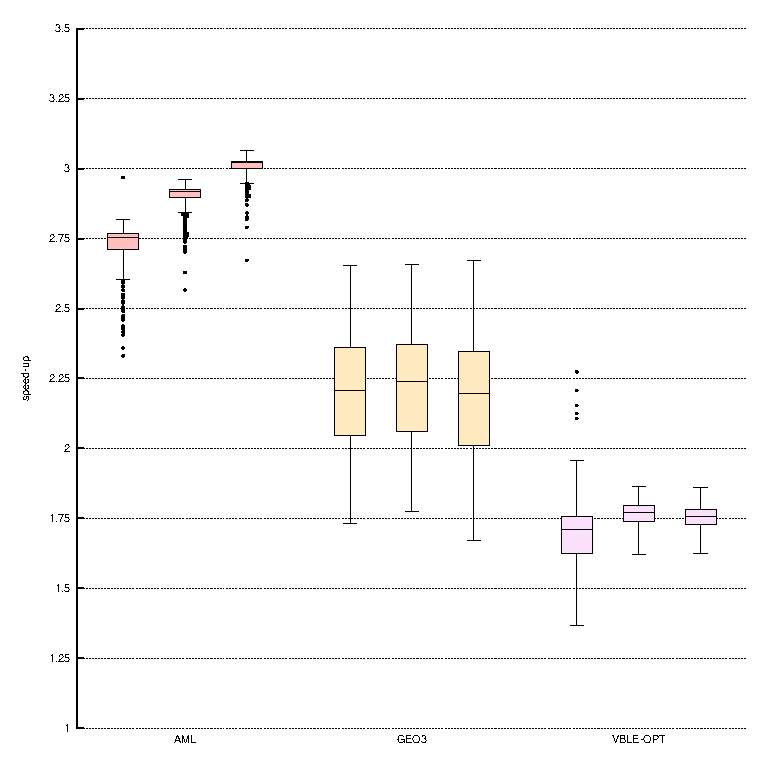
\includegraphics{img/boxplot}
\end{center}
\caption{Distribution of speed-ups}
\label{fig:boxplot}
\end{figure}

In general, it is arguable whether these average speed-ups can be used to evaluate the success of my optimizational work. The algorithms showed remarkable differences in the distribution of the test data, which can be seen in the box-and-whisker diagram in Figure~\ref{fig:boxplot}. Whereas speed-ups of AML and VBLE-OPT have a small variance, Geolateration has a considerably larger dispersion with its interquartile range spreading from around 2.05 to 2.35. I expect this to a be consequence of the many early-out conditionals contained in Geo3, which in general lead to large variances in the algorithm runtimes. Some manual investigation into the anchor placements for speed-ups both from the lower and from the upper range of results suggested that input anchors forming a large triangle (e.g., anchors lying close to distinct corners of the playing area) led to higher speed-ups, whereas small, acute-angled triangles resulted in lower speed-ups. In the latter case, the optimizational step 4, which tests whether the minimum perimeter triangle is contained in the triangle formed by the anchors, is more likely to fail and therefore the remaining parts are executed more often. This also shows that the overall speed-up of Geo3 is not cumulative over the performance improvements of the various sections: Whereas the optimization of step 5, which calculates the geometric median of the final triangle, proved highly beneficial in my experiments, the overall speed-up of the optimization is higher in cases where it is executed less frequently.

To put some visual emphasis on the distribution of the speed-ups with respect to the spread of the runtimes, Figures~\ref{fig:scatterplots}~and~\ref{fig:vblescatterplots} display scatterplots that relate the reference runtimes to the corresponding optimized runtimes, where each point represents a single pair of runtimes. The position of points relative to the x-axis shows the general variance of reference runtimes for the given 500 random benchmark runs. Additionally, the scattering of points around the line, which interpolates the expected optimized runtimes using the calculated average speed-up (i.e., it is a plot of the formula $y = \frac{x}{\texttt{average speed-up}}$), illustrates the variance of the speed-ups. For example, to verify what has been said above, the upper right region of Figure~\ref{fig:scattergeo} shows that higher runtimes of Geo3 had an lower-than-average speed-up.

\begin{figure}
\begin{center}
\subfigure[Geo3]{
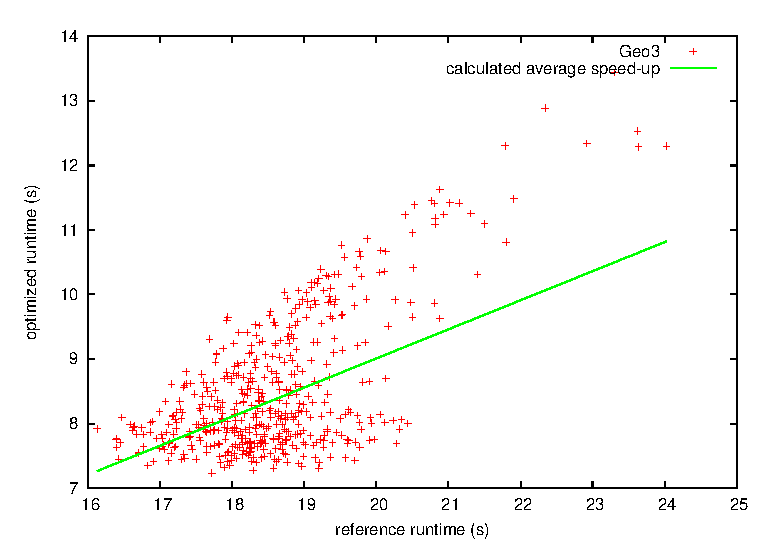
\includegraphics[width=0.75\linewidth]{img/scatter_geolat3.eps}
\label{fig:scattergeo}
}
\subfigure[AML (4 anchors)]{
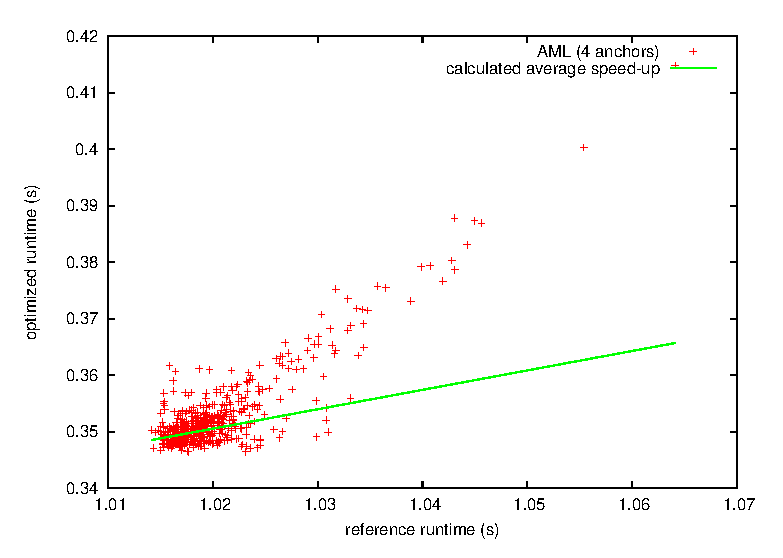
\includegraphics[width=0.75\linewidth]{img/scatter_aml4.eps}
\label{fig:scatteraml}
}
\end{center}
\caption*{\small{These scatterplots show the reference runtimes in relation to the corresponding optimized runtimes, so each point actually marks two measured values. The line is an interpolation of the \emph{calculated average speed-up}, i.e. it can be read as, ``Based on the average speed-up, one can expect a run of the algorithm that took $x$ seconds in the original implementation to take $y$ seconds in the optimized version''.}}
\caption{Scatterplots of benchmark results}
\label{fig:scatterplots}
\end{figure}

\begin{figure}
\begin{center}
\subfigure[3 anchors]{
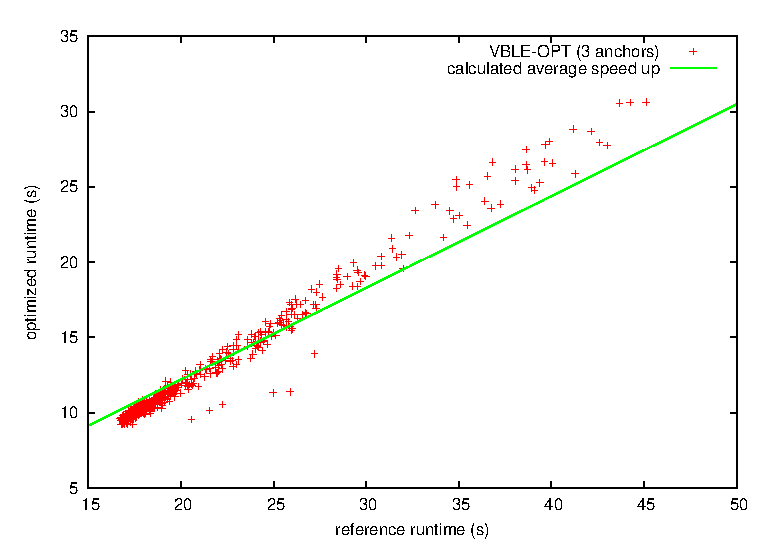
\includegraphics[width=0.75\linewidth]{img/scatter_vble3.eps}
\label{fig:scattervble3}
}
\subfigure[4 anchors]{
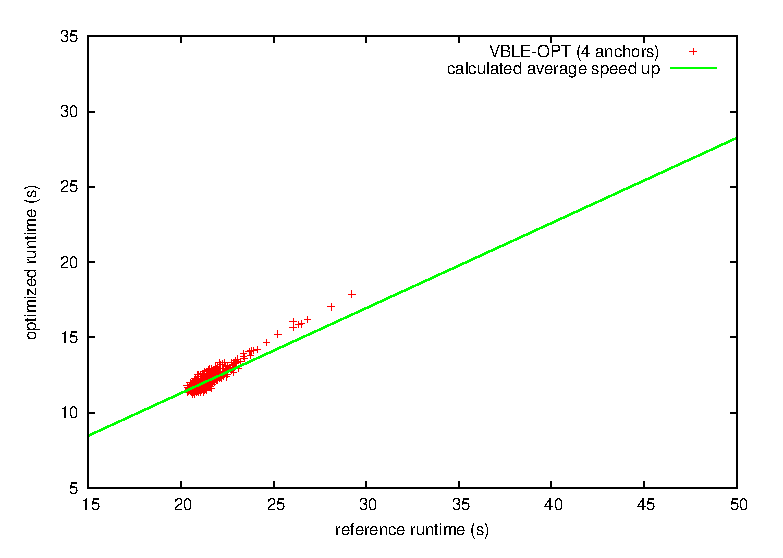
\includegraphics[width=0.75\linewidth]{img/scatter_vble4.eps}
\label{fig:scattervble4}
}
\end{center}
\caption{Benchmark results of VBLE-OPT}
\label{fig:vblescatterplots}
\end{figure}

With regards to Adapted Multilateration, although the speed-up variance is lower than in the case of Geo3, the data has only a weak empiric correlation\footnote{For an introduction to the sample correlation coefficient, see, for example,~\cite[p. 33ff]{ross2004statistics}.} of 0.172, i.e., long reference runtimes did not necessarily result in longer optimized runtimes, and vice versa. This may result from the \emph{first intersection} step occasionally needing more iterations to find circle intersections for all vector elements, in which case the benefits of the vectorization are reduced by the increased processing time spent at the vector comparisons and blending instructions Yet in other runs, the vectorization has larger impacts and runs that were previously slow turned out to have considerable shorter runtimes in the optimized implementation. The scatterplot displayed in Figure~\ref{fig:scatteraml} shows that the speed-up is quite often lower than average (i.e., above the line), yet there seems to exist no connection between the speed-ups and the original runtimes.

In view of the benchmarks of VBLE-OPT, I would like to point out that the runtimes that were measured for sets of 3 anchors differed substantially from the runtimes of benchmarks using 4 or 5 anchor (or more). Theoretically, the performance of VBLE-OPT should be almost constant with respect to the number of anchors, as the number of cells in the grid is independent of the anchor position and there are no early-out conditionals and the like. Still, when the algorithm was parametrized with 3 anchors, the runtimes varied a lot, yet only towards above the overall average (see Figure~\ref{fig:vblescatterplots}). These slower runs also showed a slightly worse speed-up factor, which resulted in a larger speed-up variance, as depicted in the box-and-whiskers diagram. The reason for these varying runtimes is still unclear to me and could be investigated in future research.

In summary, it can be stated that the outcome of the benchmarks on the whole has confirmed the positive impact of the applied SSE optimization on the performance of each algorithm. However, the methodic approach that was used to acquire these numbers contained several flaws, as described in Section~\ref{eval_approach}. Since there was a lower bound on the area of the shape formed by the anchors, a certain range of possible input shapes has not been tested. In the case of Geolateration, where the benchmarks suggest that smaller triangles have led to lower speed-up factors, this may have influenced the average speed-ups. Still, as these minimum area cases are generally not very likely, the overall tendency of the benchmarks should be correct.

\section{Conclusion}
\label{Conclusion}

What to say here?

\begin{itemize}
\item SSE wins!
\end{itemize}
\cleardoublepage
\phantomsection

% Bibliography
\addcontentsline{toc}{section}{References}
\bibliographystyle{alpha}
\bibliography{thesis}

\clearpage
\listoffigures
%\addcontentsline{toc}{section}{List of Figures}
\clearpage
\listoftables
%\addcontentsline{toc}{section}{List of Tables}
\clearpage
\lstlistoflistings
%\addcontentsline{toc}{section}{List of Listings}

\end{document}
